\documentclass[]{article}
\usepackage{lmodern}
\usepackage{amssymb,amsmath}
\usepackage{ifxetex,ifluatex}
\usepackage{fixltx2e} % provides \textsubscript
\ifnum 0\ifxetex 1\fi\ifluatex 1\fi=0 % if pdftex
  \usepackage[T1]{fontenc}
  \usepackage[utf8]{inputenc}
\else % if luatex or xelatex
  \ifxetex
    \usepackage{mathspec}
  \else
    \usepackage{fontspec}
  \fi
  \defaultfontfeatures{Ligatures=TeX,Scale=MatchLowercase}
\fi
% use upquote if available, for straight quotes in verbatim environments
\IfFileExists{upquote.sty}{\usepackage{upquote}}{}
% use microtype if available
\IfFileExists{microtype.sty}{%
\usepackage{microtype}
\UseMicrotypeSet[protrusion]{basicmath} % disable protrusion for tt fonts
}{}
\usepackage[margin=1in]{geometry}
\usepackage{hyperref}
\hypersetup{unicode=true,
            pdftitle={Project MSG500-MVE190 Linear Statistical Models},
            pdfauthor={Stefan Eng \& Masood Bagheri},
            pdfborder={0 0 0},
            breaklinks=true}
\urlstyle{same}  % don't use monospace font for urls
\usepackage{longtable,booktabs}
\usepackage{graphicx,grffile}
\makeatletter
\def\maxwidth{\ifdim\Gin@nat@width>\linewidth\linewidth\else\Gin@nat@width\fi}
\def\maxheight{\ifdim\Gin@nat@height>\textheight\textheight\else\Gin@nat@height\fi}
\makeatother
% Scale images if necessary, so that they will not overflow the page
% margins by default, and it is still possible to overwrite the defaults
% using explicit options in \includegraphics[width, height, ...]{}
\setkeys{Gin}{width=\maxwidth,height=\maxheight,keepaspectratio}
\IfFileExists{parskip.sty}{%
\usepackage{parskip}
}{% else
\setlength{\parindent}{0pt}
\setlength{\parskip}{6pt plus 2pt minus 1pt}
}
\setlength{\emergencystretch}{3em}  % prevent overfull lines
\providecommand{\tightlist}{%
  \setlength{\itemsep}{0pt}\setlength{\parskip}{0pt}}
\setcounter{secnumdepth}{0}
% Redefines (sub)paragraphs to behave more like sections
\ifx\paragraph\undefined\else
\let\oldparagraph\paragraph
\renewcommand{\paragraph}[1]{\oldparagraph{#1}\mbox{}}
\fi
\ifx\subparagraph\undefined\else
\let\oldsubparagraph\subparagraph
\renewcommand{\subparagraph}[1]{\oldsubparagraph{#1}\mbox{}}
\fi

%%% Use protect on footnotes to avoid problems with footnotes in titles
\let\rmarkdownfootnote\footnote%
\def\footnote{\protect\rmarkdownfootnote}

%%% Change title format to be more compact
\usepackage{titling}

% Create subtitle command for use in maketitle
\newcommand{\subtitle}[1]{
  \posttitle{
    \begin{center}\large#1\end{center}
    }
}

\setlength{\droptitle}{-2em}

  \title{Project MSG500-MVE190 Linear Statistical Models}
    \pretitle{\vspace{\droptitle}\centering\huge}
  \posttitle{\par}
    \author{Stefan Eng \& Masood Bagheri}
    \preauthor{\centering\large\emph}
  \postauthor{\par}
    \date{}
    \predate{}\postdate{}
  

\begin{document}
\maketitle

\subsection{Introduction}\label{introduction}

We are considering a dataset that provides some demographic information
for 440 of the most populous counties in the United States in years
1990-92. Each line of the dataset provides information on 14 variables
for a single county. Counties with missing data were deleted from the
dataset. We are building models to predict the number of crimes per 1000
people in each county. We first explore linear regression models and
then a negative binomial regression model. We found that the best linear
regression model performed similarly to the negative binomial regression
model on the training and test set using the same variables.

\subsection{Goals}\label{goals}

The goals of the analysis was the find a model that is simple yet
explains as much as possible. The model should make sense first and
foremost. Automatic methods such as the backwards step algorithm were
used as auxiliary methods to supplement a more hand selected model. We
decided against using all possible subsets selection as a matter of
principle as it can lead to models that lack explainability. We explore
interactions between variables as well as standard additive models. Once
model selection is done based on the training set the final results are
reported against the test set (20\% of the dataset). The test set was
not looked at or used in the model building process. The models were
compared on the training set using 10-fold cross validation and leave
one out cross validation (LOOCV).

\subsection{Data Processing}\label{data-processing}

Some additional variables were created. The variables ``beds'',
``phys'', and ``area'' were all divide by the population to give a per
capita total number of hospital beds, cribs and bassinets, per capita
number of physicians practicing, and the per capita area. We then remove
the total quantities from the data set. We found that working with per
capita was more informative than the direct quantities. The data was
also transformed almost entirely with natural log transform as it
performed better for our model. We arrived at natural log based on the
plots, residuals plots, and looking how the model's \(R^2\) changed with
regard to the transformations along with cross validation. The data
summary can be found in the appendix.

\subsection{Models}\label{models}

\subsubsection{Full Model}\label{full-model}

\begin{verbatim}
crm1000 ~ percapitaarea + popul + pop1834 + pop65plus +
          percapitaphys + percapitabeds + higrads + bachelors +
          poors + unemployed + percapitaincome + region
\end{verbatim}

The full model was used as a baseline model, and subsequent models were
reduced from this model.

\paragraph{Base Model}\label{base-model}

\begin{verbatim}
crm1000 ~ percapitaarea + popul + pop1834 +
          percapitabeds + poors + percapitaincome + region
\end{verbatim}

These are the variables from which all the other models are based. We
arrived at this model by keeping one variable from each correlation
cluster that seemed to make the most intuitive sense to keep. We
confirmed that this was a good model by starting with all of the
variables and using backward selection to arrive at the identicial model
that we had selected by hand. Then a partial F-test was performed, see
table below. The F statistic was extremely small, which means that the
residual sum of squares was almost the same after dropping the variables
\texttt{pop65plus}, \texttt{percapitaphys}, \texttt{higrads},
\texttt{bachelors}, and \texttt{unemployed}. From this reduced model, we
built up variations that involved transformations and interactions.

\begin{longtable}[]{@{}rrrrrr@{}}
\caption{Partial F-Test for Full model vs final model (without
transformations)}\tabularnewline
\toprule
Res.Df & RSS & Df & Sum of Sq & F & Pr(\textgreater{}F)\tabularnewline
\midrule
\endfirsthead
\toprule
Res.Df & RSS & Df & Sum of Sq & F & Pr(\textgreater{}F)\tabularnewline
\midrule
\endhead
337 & 143366.5 & NA & NA & NA & NA\tabularnewline
342 & 144262.2 & -5 & -895.74 & 0.421 & 0.834\tabularnewline
\bottomrule
\end{longtable}

\subsubsection{(Final Model) Log Transformed model with no
interactions}\label{final-model-log-transformed-model-with-no-interactions}

This model ended up being our final model selection. The transformation
were found through cross validation and analysis of the plots of the
data.

\begin{verbatim}
crm1000 ~ log(percapitaarea) + log(popul) + log(pop1834) +
          log(percapitabeds) + log(poors) + log(percapitaincome) + region
\end{verbatim}

\subsubsection{Transformations and Interactions with only
region.}\label{transformations-and-interactions-with-only-region.}

We included all interactions between the continuous variables and the
region. We then backward selected that reduced to (log) population and
(log) per capita income against the region. While running the backwards
selection we checked that the main effects were not dropped while the
interactions were kept.

\begin{verbatim}
crm1000 ~ log(percapitaarea) + log(popul) + log(pop1834) +
          log(percapitabeds) + log(poors) + log(percapitaincome) +
          region + log(popul):region + log(percapitaincome):region
\end{verbatim}

\subsubsection{Transformations and Interactions against all
variables.}\label{transformations-and-interactions-against-all-variables.}

We included the interactions between all variables (including
continuous-continuous) then backward selected. Both of the interactions
models included \texttt{log(popul):region} but the larger interaction
model did not include \texttt{log(percapitaincome):region}. We suspect
this may be from the correlation between per capita income and some of
the other variables that are included such as the percentage of poor
people.

\begin{verbatim}
crm1000 ~ log(percapitaarea) + log(popul) + log(pop1834) +
          log(percapitabeds) + log(poors) + log(percapitaincome) +
          region + log(popul):log(percapitabeds) +
          log(popul):log(poors) + log(popul):log(percapitaincome) +
          log(popul):region + log(pop1834):region +
          log(percapitabeds):region + log(poors):log(percapitaincome) +
          log(poors):region
\end{verbatim}

\subsubsection{Negative Binomial Generalized Linear
Model}\label{negative-binomial-generalized-linear-model}

We used the same variables from the log transformed model with no
interactions. Instead of modeling crime rate per 1000 people directly we
model the crimes. We use an offset to adjust the parameters according to
the population (more is described in Negative Binomial Model section).

\begin{verbatim}
crimes ~ offset(log(popul / 1000)) + log(percapitaarea) +
         log(popul) + log(pop1834) + log(percapitabeds) +
         log(poors) + log(percapitaincome) + region
\end{verbatim}

\subsubsection{Other models}\label{other-models}

For our cross-validation and model selection we included two models
which we did not intend to use but only for comparision purposes. They
were the full model which was described above. Also, we included a model
which we call the \emph{simple model} which only included the natural
log of the percentage of poor people in the county.

\subsection{Multicollinearity}\label{multicollinearity}

In this dataset there are many variables that are highly correlated (see
appendix for correlation plot). We found that the percentage of poor
people in a county was highly correlated with the per capita income and
the number of high school grads. If we include all of the variables with
high multicollinearity the standard errors will be increased and some of
the variables may not end up being significant. We used the Variance
inflation factor (VIF) to measure the multicollinearity in our model.
The VIF is the ratio of variance in a model with multiple terms, divided
by the variance of a model with one term alone (CITE ISL). This gives us
a measure of how much the coefficient's variance will increase due to
collinearity between the other variables. The VIF factors are the
computed by regressing all the other explanatory variables on a single
variable \(x_i\). The VIF factor is equal to \[
VIF_i = \frac{1}{1 - R_i^2}
\] We removed the variables for per capita income, the number of high
school graduates, and the number of bachelor degree graduates based on
the VIF results. The last column in the table shows how much the
standard error of the variable is increased due to the collinearity. For
example, for the bachelors variable the value of 2.834 means that the
standard error for \(\beta_{bachelors}\) is 2.834 larger than if the
variables were not correlated with each other.

\begin{longtable}[]{@{}lrrr@{}}
\toprule
& VIF & DF & VIF\^{}(1/(2*Df))\tabularnewline
\midrule
\endhead
bachelors & 8.030 & 1 & 2.834\tabularnewline
percapitaincome & 5.207 & 1 & 2.282\tabularnewline
higrads & 4.899 & 1 & 2.213\tabularnewline
poors & 4.162 & 1 & 2.040\tabularnewline
percapitabeds & 3.309 & 1 & 1.819\tabularnewline
percapitaphys & 3.022 & 1 & 1.738\tabularnewline
region & 2.847 & 3 & 1.191\tabularnewline
pop1834 & 2.742 & 1 & 1.656\tabularnewline
unemployed & 2.157 & 1 & 1.469\tabularnewline
pop65plus & 2.123 & 1 & 1.457\tabularnewline
percapitaarea & 1.553 & 1 & 1.246\tabularnewline
popul & 1.290 & 1 & 1.136\tabularnewline
\bottomrule
\end{longtable}

\subsection{Outliers}\label{outliers}

When looking at the training data we noticed one outlier with respect to
the target variable in the training dataset (Kings County in New York).
It has a crime rate of approximately 296 per 1000 people. The median for
the training set was a crime rate of 53.55 per 1000 people. In the
training set we found that Kings County has larger leverage and also has
high influence. There are also outliers with respect to the other
variables but the amount is reduced when we took the log transform of
the data. In the appendix, we go into more detailed look at other
outliers based on the studentized residuals and influence.

\subsection{Interactions}\label{interactions}

We explored and built models that included interactions between the
variables. We found that while some of the interactions were
significant, when doing cross validation the additive model without any
interactions performed the best. Using the partial F-test, we compared
the two interaction models with the additive model. For the interactions
model with only region, we did not reject the null hypothesis at the
\(\alpha = 0.05\) level, as the p-value was 0.06. The value was close
enough that we decided to continue to compare with this model as well.
The results can be see in the table below. When we run a partial F-test
on the interaction models with more interactions, we get a larger test
statistic that allows us to reject the null hypothesis at the
\(\alpha = 0.05\) level.

\begin{longtable}[]{@{}rrrrrr@{}}
\caption{Partial F-test for region interactions model}\tabularnewline
\toprule
Res.Df & RSS & Df & Sum of Sq & F & Pr(\textgreater{}F)\tabularnewline
\midrule
\endfirsthead
\toprule
Res.Df & RSS & Df & Sum of Sq & F & Pr(\textgreater{}F)\tabularnewline
\midrule
\endhead
342 & 124062.3 & NA & NA & NA & NA\tabularnewline
336 & 119758.2 & 6 & 4304.037 & 2.013 & 0.063\tabularnewline
\bottomrule
\end{longtable}

\begin{longtable}[]{@{}rrrrrr@{}}
\caption{Partial F-test for full interactions model}\tabularnewline
\toprule
Res.Df & RSS & Df & Sum of Sq & F & Pr(\textgreater{}F)\tabularnewline
\midrule
\endfirsthead
\toprule
Res.Df & RSS & Df & Sum of Sq & F & Pr(\textgreater{}F)\tabularnewline
\midrule
\endhead
342 & 124062.3 & NA & NA & NA & NA\tabularnewline
326 & 105258.6 & 16 & 18803.67 & 3.639842 & 4e-06\tabularnewline
\bottomrule
\end{longtable}

In the conditional plot we can see the values of the log of population
vs the crime rate for each of the regions. The bottom left panel is the
West, bottom right is the northeast, top left is the midwest and top
right is the south. There seems to be a slightly smaller slope in the
West panel, but overall it is not clear that the interactions are
needed.

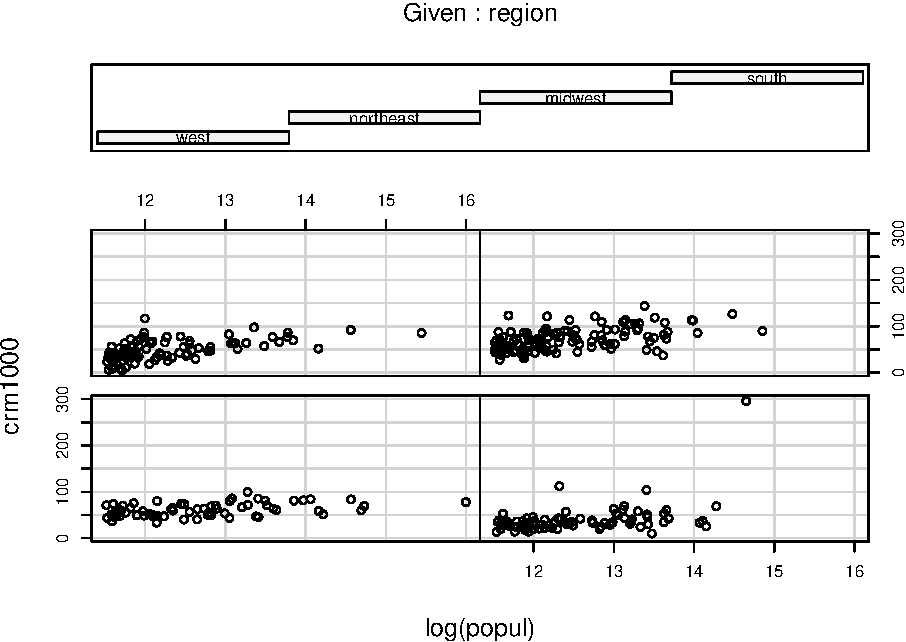
\includegraphics{project_files/figure-latex/unnamed-chunk-7-1.pdf}

Our original cross validation was performed on data that was not
centered (mean subtracted off). Centering can improve the standard
errors and thus the p-values of the estimates but the predictions for
the new values are the same. Since our final model does not include the
interactions, we decided against centering the data. When building the
interaction models we included all of the interactions (for region and
then for all variables) and then backward selected. We did this twice:
once with the data centered and once without the data being centered.
While this does not make a difference for the estimate, the standard
errors decrease in the centered model. That made the backwards selection
algorithm stop earlier when we centered the data, and thus included more
of the interaction variables. Again, at this point we checked to make
sure that no interaction effects were included when a main effect was
dropped. When including these centered models in our cross validation we
found that they performed worse than the backward selection models on
the original (non-standardized) data so we chose not to include them in
our analysis.

\subsection{Model Interpretation}\label{model-interpretation}

On the training data, we had an \(R^2\) of 0.543 which means that 54.3\%
of the error is explained by our model. The \(R_{adj}^2\) was 0.531.

\begin{longtable}[]{@{}lrrr@{}}
\toprule
& Estimate & Std. Error &
Pr(\textgreater{}\textbar{}t\textbar{})\tabularnewline
\midrule
\endhead
(Intercept) & -372.847 & 108.328 & 0.001\tabularnewline
log(percapitaarea) & -5.127 & 1.494 & 0.001\tabularnewline
log(popul) & 5.725 & 1.970 & 0.004\tabularnewline
log(pop1834) & 17.534 & 7.813 & 0.025\tabularnewline
log(percapitabeds) & 3.625 & 2.454 & 0.141\tabularnewline
log(poors) & 25.475 & 3.932 & 0.000\tabularnewline
log(percapitaincome) & 24.893 & 9.948 & 0.013\tabularnewline
regionnortheast & -18.548 & 3.830 & 0.000\tabularnewline
regionmidwest & -10.724 & 3.761 & 0.005\tabularnewline
regionsouth & 4.974 & 3.453 & 0.151\tabularnewline
\bottomrule
\end{longtable}

Let's look at what these estimates actually mean. Since we are working
on a log scale we can interpret the estimate \(\beta_{area}\) for
log(percapitaarea) as the change in crime rate per 1000, \(crm_{1000}\),
when \(log(percapitaarea)\) increases by 1. That is,
\(\ln x_{area} + 1 = \ln(e \cdot x_{area})\). So if \(x_{area}\) is
\emph{multiplied} by \(e \approx 2.718\), then \(crm_{1000}\) increases
by \(\beta_{area}\). It can be easier to interpret if we look at
percentage increase instead of multiplying by \(e\). If the per captia
area increases by 10\%, then the crime rate per 1000 people will
\emph{decrease} by 0.49.
\(\beta_{area} \cdot ln(1.10) = -5.127 \cdot ln(1.10) = -0.49\). This is
summarized in the table

\begin{longtable}[]{@{}lrrrr@{}}
\caption{Change in crime rate by percentage increase}\tabularnewline
\toprule
& 5\% & 10\% & 20\% & 30\%\tabularnewline
\midrule
\endfirsthead
\toprule
& 5\% & 10\% & 20\% & 30\%\tabularnewline
\midrule
\endhead
percapitaarea & -0.250 & -0.489 & -0.935 & -1.345\tabularnewline
popul & 0.279 & 0.546 & 1.044 & 1.502\tabularnewline
pop1834 & 0.855 & 1.671 & 3.197 & 4.600\tabularnewline
percapitabeds & 0.177 & 0.346 & 0.661 & 0.951\tabularnewline
poors & 1.243 & 2.428 & 4.645 & 6.684\tabularnewline
percapitaincome & 1.215 & 2.373 & 4.538 & 6.531\tabularnewline
\bottomrule
\end{longtable}

From this table we can see that if the the percentage of poor people
increased from 20 to 22, we would expect to see an increase of 2.428 in
the number of crimes per 1000 people. We can also see that if the per
captia area increases from \(5 \times 10^{-3}\) to
\(5.5 \times 10^{-3}\) we would expect the number of crimes per 1000
people to \emph{drop} by 0.489.

\subsubsection{Region}\label{region}

We used ``West'' as our reference category so all the parameter
estimates are in relation to the west region. We can interpret the
estimate \(\beta_{region_{NE}} = -18.548\) as the estimate change in
crimes per 1000 people between the west and the north east. That is,
holding all else constant, the north-east region is estimated to have
\(18.548\) less crimes per 1000 people. Both the north-east and the
midwest are statistically significant at the \(\alpha = 0.05\) level.
The difference between the south and the west's rate of crimes is not
statistically significant. That means that the there is not enough
evidence from the data to show there is a difference in crime rates
between the south and the west (assuming all else is held constant).

\subsection{Negative Binomial Model}\label{negative-binomial-model}

We also explored generalized linear models for predicting the crime
rate. Since we are dealing with the rate \(1000 * crimes/popul\), we can
formulate our model as

\[
log(crimes) = log(popul/1000) + X\beta
\]

Since we are using the (log) population in our model, having an offset
is equivalent to the value of the coefficient for log(population) will
increased by 1, and the intercept decreased by log(1000). We first
tested a Poisson regression which assumed that the variance and expected
value are the same for the crimes. When performing a dispersion test at
\(\alpha = 0.05\), we rejected the null that dispersion is equal to one.
(Estimated dispersion was 2622.163). When dispersion is greater than
one, we say that the data is overdispersed. The negative binomial model
works better in the presence of overdispersion.

\subsubsection{Interpreting Results}\label{interpreting-results}

\begin{longtable}[]{@{}lrr@{}}
\toprule
& Estimate & p-value\tabularnewline
\midrule
\endhead
(Intercept) & -3.569 & 0.052\tabularnewline
log(percapitaarea) & -0.072 & 0.004\tabularnewline
log(popul) & 0.096 & 0.004\tabularnewline
log(pop1834) & 0.336 & 0.011\tabularnewline
log(percapitabeds) & 0.097 & 0.020\tabularnewline
log(poors) & 0.414 & 0.000\tabularnewline
log(percapitaincome) & 0.477 & 0.005\tabularnewline
regionnortheast & -0.468 & 0.000\tabularnewline
regionmidwest & -0.243 & 0.000\tabularnewline
regionsouth & 0.043 & 0.462\tabularnewline
\bottomrule
\end{longtable}

We can interpret the results from negative binomial similarly to Poisson
regression. Let's look at how the percentage of poor people in a county
influences the number of crimes. We have that \[
\log(crimes) = \beta_0 + \beta_{poors} \log x_{poors} + \cdots
\] or \[
crimes = \exp(\beta_0 + \beta_{poors} \log x_{poors}  + \cdots) = e^{\beta_0} x_{poors}^{\beta_{poors}} \cdots
\] Now if we want to see what happens as \(x_{poors}\) changes, say to
\(x_{poors}^{\prime}\), then we have that \[
\frac{crimes^{\prime}}{crimes} = \left(\frac{x_{poors}^{\prime}}{x_{poors}}\right)^{\beta_{poors}}
\] That is, the percentage change in the crimes is equal to the
percentage change in percentage of poor people to the power of the
coefficient for poors. Equivalently we pose this additively as \[
\log crimes^{\prime} - \log crimes = \beta_{poors} \left( \log x_{poors}^{\prime} - \log x_{poors} \right)
\] So if we kept all other variables constant, and increased
\(x_{poors}\) from 10 to 12 we would expect: \[
\frac{crimes^{\prime}}{crimes} = \left(\frac{12}{10} \right)^{0.414} = 1.078
\] That is, we would expect the crimes to increase by 7.8\%. We can
confirm this for the predicted crimes per 1000 people while holding all
other variables at the means. When \(x_{poors} = 10\), then the
predicted crime rate is 71.68. The predicted crime from for
\(x_{poors} = 12\) is 77.3. The ratio of these values is 1.078 which is
what we found from the coefficient interpretation.

It is also useful to look at how the predicts change as one of the
variables varies. We set all of the variables involved in the regression
to the means and then only varied the percentage of poor from 1 to 37,
which is approximately the range found in the training set. It is easier
to see how the crime rate changes from this graph due to the poor
percentage changing than just the estimated coefficients.
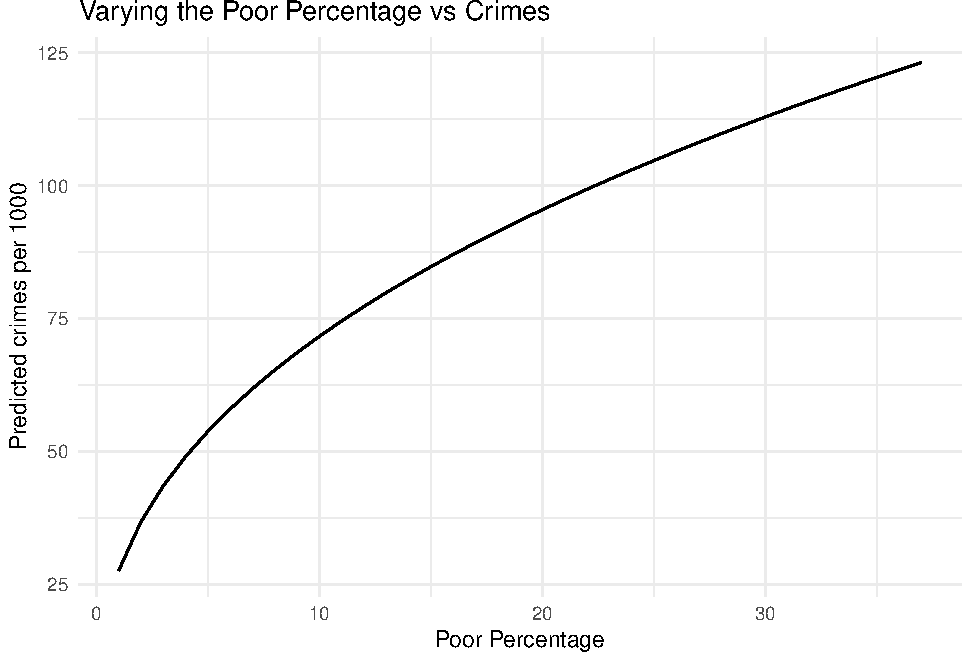
\includegraphics{project_files/figure-latex/unnamed-chunk-12-1.pdf}

\subsection{Cross Validation}\label{cross-validation}

Once we had built our models we used 10-fold cross validation to compare
them against each other. We also used LOOCV which resulted in very
similar results to the 10-fold cross validation. Once we had included
the negative binomial model we switched to only using the 10-fold cross
validation. The interactions models had a better adjusted \(R^2\) value
and were found with the partial F-test to have at least one parameters
that should not be set to 0 (at alpha = 0.05 significance level). We
included a model called ``Full'', which had all of the dependent
variables included (without transformation) and a ``simple'' model which
is only using the natural log of the percentage of poor people for each
county.

\begin{longtable}[]{@{}rrrrrr@{}}
\caption{Average MSE across 10-folds}\tabularnewline
\toprule
Additive & NB & RegionInter & AllInter & Full & Simple\tabularnewline
\midrule
\endfirsthead
\toprule
Additive & NB & RegionInter & AllInter & Full & Simple\tabularnewline
\midrule
\endhead
395.69 & 415.05 & 430.86 & 439.82 & 500.43 & 605.53\tabularnewline
\bottomrule
\end{longtable}

\subsection{Test Validation}\label{test-validation}

At this point of the analysis everything had been conducted on the
training 80\% of the dataset. Cross validation was used as part of the
model building process which means that the results will be biased. We
kept the test set held out until the end when all models were finalized
so that the estimated mean squared error is a better indication of the
true mean squared error. The results on the test sets are as follows

\begin{longtable}[]{@{}rrrrrr@{}}
\caption{Test MSE will all data from test included}\tabularnewline
\toprule
Additive & NB & RegionInter & AllInter & Full & Simple\tabularnewline
\midrule
\endfirsthead
\toprule
Additive & NB & RegionInter & AllInter & Full & Simple\tabularnewline
\midrule
\endhead
235.61 & 236.57 & 248.13 & 269.4 & 309.62 & 471.37\tabularnewline
\bottomrule
\end{longtable}

\begin{longtable}[]{@{}rrrrrr@{}}
\caption{Test MSE with Kings County excluded}\tabularnewline
\toprule
NB & Additive & AllInter & RegionInter & Full & Simple\tabularnewline
\midrule
\endfirsthead
\toprule
NB & Additive & AllInter & RegionInter & Full & Simple\tabularnewline
\midrule
\endhead
248.82 & 252.86 & 256.69 & 256.73 & 310.86 & 469.59\tabularnewline
\bottomrule
\end{longtable}

We can see that including Kings County (NY) leads to slightly better
results in the test set. Based on these results, we can see that both
the negative binomial and the additive model without interactions
performs the best and almost identically. Since linear regression is
faster and simpler to interpret the results our final model is the Log
Transformed model with no interactions, in the models section.

Using this as our final model, we can fit this model to the test
selection data. This can be seen as a more conservative approach to our
parameters since it is on the test set rather than the training.

\begin{longtable}[]{@{}lrrr@{}}
\caption{Test set coefficients and p-values}\tabularnewline
\toprule
& Estimate & Std. Error &
Pr(\textgreater{}\textbar{}t\textbar{})\tabularnewline
\midrule
\endfirsthead
\toprule
& Estimate & Std. Error &
Pr(\textgreater{}\textbar{}t\textbar{})\tabularnewline
\midrule
\endhead
(Intercept) & -385.074 & 183.899 & 0.040\tabularnewline
log(percapitaarea) & -4.265 & 2.431 & 0.083\tabularnewline
log(popul) & 8.626 & 3.467 & 0.015\tabularnewline
log(pop1834) & 23.087 & 10.855 & 0.037\tabularnewline
log(percapitabeds) & 8.167 & 4.689 & 0.086\tabularnewline
log(poors) & 24.635 & 6.459 & 0.000\tabularnewline
log(percapitaincome) & 23.818 & 16.421 & 0.151\tabularnewline
regionnortheast & -20.565 & 7.189 & 0.005\tabularnewline
regionmidwest & -6.943 & 7.233 & 0.340\tabularnewline
regionsouth & 3.083 & 6.712 & 0.647\tabularnewline
\bottomrule
\end{longtable}

We have \(R^2_{adj} =\) 0.614 and \(R^2 =\) 0.654. Which means that
\texttt{round(sm\_final\$r.squared\ *\ 100,2)} percent of the error is
explained by our model. The p-values in this table are the most
conservative, since we have not seen any of the data when testing this
hypothesis. In this way, it is like a properly run experiment. We do not
want to fish for statistically significance by creating hypotheses based
on our data set. Instead if we formulate our hypothesis beforehand we
should use the data set to validate our hypothesis.

\subsubsection{Final Coefficients}\label{final-coefficients}

Combining the training and test data sets and fitting our final model on
this gives us our final coefficients. We want to use all the data if we
are going to predict for more counties in the future. We can interpret
these estimates exactly the same as for the training and test data. The
p-values are artificially low, due to a large sample size and the fact
that 80\% of the data is from the training set which we used to
generated the hypothesis.

\begin{longtable}[]{@{}lrrr@{}}
\caption{Final coefficients and p-values}\tabularnewline
\toprule
& Estimate & Std. Error &
Pr(\textgreater{}\textbar{}t\textbar{})\tabularnewline
\midrule
\endfirsthead
\toprule
& Estimate & Std. Error &
Pr(\textgreater{}\textbar{}t\textbar{})\tabularnewline
\midrule
\endhead
(Intercept) & -387.885 & 92.606 & 0.000\tabularnewline
log(percapitaarea) & -5.009 & 1.276 & 0.000\tabularnewline
log(popul) & 6.108 & 1.697 & 0.000\tabularnewline
log(pop1834) & 18.891 & 6.415 & 0.003\tabularnewline
log(percapitabeds) & 4.327 & 2.163 & 0.046\tabularnewline
log(poors) & 25.606 & 3.345 & 0.000\tabularnewline
log(percapitaincome) & 25.910 & 8.400 & 0.002\tabularnewline
regionnortheast & -18.795 & 3.311 & 0.000\tabularnewline
regionmidwest & -9.823 & 3.303 & 0.003\tabularnewline
regionsouth & 4.531 & 3.009 & 0.133\tabularnewline
\bottomrule
\end{longtable}

We find it easier to understand some of these estimates with plots.
Below we show how the predicted crime rates change when holding all
variables constant while varying only the population. We range the
population from the minimum 100043 to the maximum 8863164.

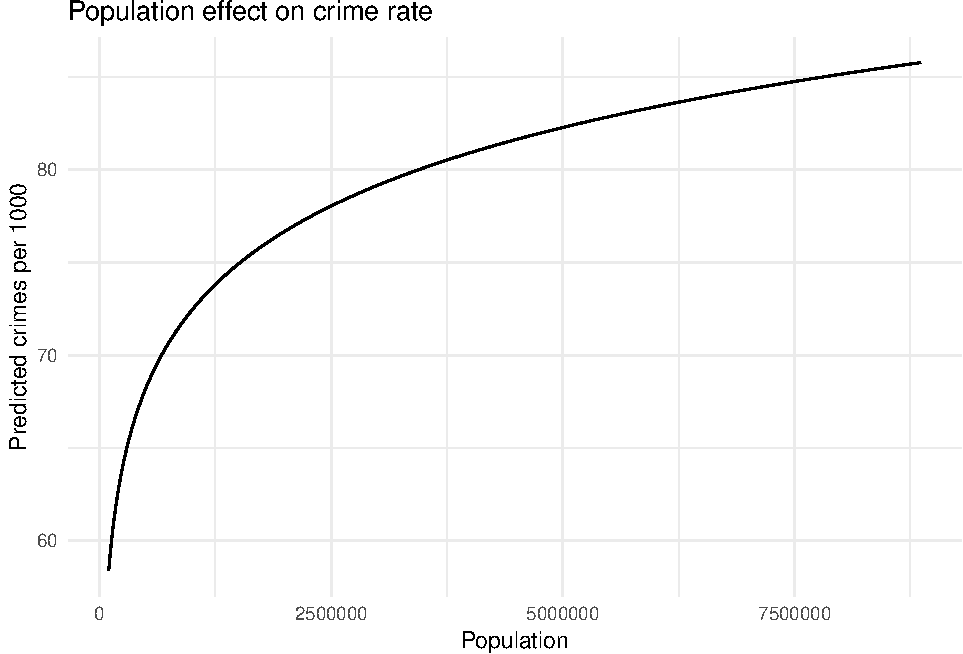
\includegraphics{project_files/figure-latex/unnamed-chunk-18-1.pdf}

\subsection{Conclusion}\label{conclusion}

In this analysis we investigated the crime rates for 440 counties in the
United States. The dataset was split into 80\% training data and 20\%
test data. The test dataset was untouched until all models were
finalized. We compared multiple linear regression models and a negative
binomial model and compared the results. The models were compared using
10-fold cross validation as part of the model building process as well
as for validation. The most predictive variables in the data set were
the population, the percentage of the population between 18 and 34, the
per captia beds, the percentage of poor people, the per capita income,
and the region in the United States. We showed that the difference
between West and Northeast crime rate had a statistically significant
difference and well as the difference between West and Midwest.

\subsection{Appendix}\label{appendix}

\subsubsection{Data Summary}\label{data-summary}

\begin{longtable}[]{@{}ll@{}}
\toprule
\begin{minipage}[b]{0.11\columnwidth}\raggedright\strut
Variable\strut
\end{minipage} & \begin{minipage}[b]{0.84\columnwidth}\raggedright\strut
Description\strut
\end{minipage}\tabularnewline
\midrule
\endhead
\begin{minipage}[t]{0.11\columnwidth}\raggedright\strut
id\strut
\end{minipage} & \begin{minipage}[t]{0.84\columnwidth}\raggedright\strut
identification number, 1--440.\strut
\end{minipage}\tabularnewline
\begin{minipage}[t]{0.11\columnwidth}\raggedright\strut
county\strut
\end{minipage} & \begin{minipage}[t]{0.84\columnwidth}\raggedright\strut
county name.\strut
\end{minipage}\tabularnewline
\begin{minipage}[t]{0.11\columnwidth}\raggedright\strut
state\strut
\end{minipage} & \begin{minipage}[t]{0.84\columnwidth}\raggedright\strut
state abbreviation.\strut
\end{minipage}\tabularnewline
\begin{minipage}[t]{0.11\columnwidth}\raggedright\strut
area\strut
\end{minipage} & \begin{minipage}[t]{0.84\columnwidth}\raggedright\strut
land area (square miles).\strut
\end{minipage}\tabularnewline
\begin{minipage}[t]{0.11\columnwidth}\raggedright\strut
popul\strut
\end{minipage} & \begin{minipage}[t]{0.84\columnwidth}\raggedright\strut
estimated 1990 population.\strut
\end{minipage}\tabularnewline
\begin{minipage}[t]{0.11\columnwidth}\raggedright\strut
pop1834\strut
\end{minipage} & \begin{minipage}[t]{0.84\columnwidth}\raggedright\strut
percent of 1990 CDI population aged 18--34.\strut
\end{minipage}\tabularnewline
\begin{minipage}[t]{0.11\columnwidth}\raggedright\strut
pop65plus\strut
\end{minipage} & \begin{minipage}[t]{0.84\columnwidth}\raggedright\strut
percent of 1990 CDI population aged 65 years old or older.\strut
\end{minipage}\tabularnewline
\begin{minipage}[t]{0.11\columnwidth}\raggedright\strut
phys\strut
\end{minipage} & \begin{minipage}[t]{0.84\columnwidth}\raggedright\strut
number of professionally active nonfederal physicians during 1990.\strut
\end{minipage}\tabularnewline
\begin{minipage}[t]{0.11\columnwidth}\raggedright\strut
beds\strut
\end{minipage} & \begin{minipage}[t]{0.84\columnwidth}\raggedright\strut
total number of hospital beds, cribs and bassinets during 1990.\strut
\end{minipage}\tabularnewline
\begin{minipage}[t]{0.11\columnwidth}\raggedright\strut
crimes\strut
\end{minipage} & \begin{minipage}[t]{0.84\columnwidth}\raggedright\strut
total number of serious crimes in 1990 (including murder, rape, robbery,
aggravated assault, burglary, larceny-theft, motor vehicle theft).\strut
\end{minipage}\tabularnewline
\begin{minipage}[t]{0.11\columnwidth}\raggedright\strut
higrads\strut
\end{minipage} & \begin{minipage}[t]{0.84\columnwidth}\raggedright\strut
percent of adults (25 yrs old or older) who completed at least 12 years
of school.\strut
\end{minipage}\tabularnewline
\begin{minipage}[t]{0.11\columnwidth}\raggedright\strut
bachelors\strut
\end{minipage} & \begin{minipage}[t]{0.84\columnwidth}\raggedright\strut
percent of adults (25 yrs old or older) with bachelor's degree.\strut
\end{minipage}\tabularnewline
\begin{minipage}[t]{0.11\columnwidth}\raggedright\strut
poors\strut
\end{minipage} & \begin{minipage}[t]{0.84\columnwidth}\raggedright\strut
Percent of 1990 CDI population with income below poverty level.\strut
\end{minipage}\tabularnewline
\begin{minipage}[t]{0.11\columnwidth}\raggedright\strut
unemployed\strut
\end{minipage} & \begin{minipage}[t]{0.84\columnwidth}\raggedright\strut
percent of 1990 CDI labor force which is unemployed.\strut
\end{minipage}\tabularnewline
\begin{minipage}[t]{0.11\columnwidth}\raggedright\strut
percapitaincome\strut
\end{minipage} & \begin{minipage}[t]{0.84\columnwidth}\raggedright\strut
per capita income of 1990 CDI population (dollars).\strut
\end{minipage}\tabularnewline
\begin{minipage}[t]{0.11\columnwidth}\raggedright\strut
totalincome\strut
\end{minipage} & \begin{minipage}[t]{0.84\columnwidth}\raggedright\strut
total personal income of 1990 CDI population (in millions of
dollars).\strut
\end{minipage}\tabularnewline
\begin{minipage}[t]{0.11\columnwidth}\raggedright\strut
region\strut
\end{minipage} & \begin{minipage}[t]{0.84\columnwidth}\raggedright\strut
Geographic region classification used by the U.S. Bureau of the Census,
where 1=Northeast, 2 = Midwest, 3=South, 4=West.1\strut
\end{minipage}\tabularnewline
\begin{minipage}[t]{0.11\columnwidth}\raggedright\strut
percapitabeds\strut
\end{minipage} & \begin{minipage}[t]{0.84\columnwidth}\raggedright\strut
number of beds (see descriptions above) per capita\strut
\end{minipage}\tabularnewline
\begin{minipage}[t]{0.11\columnwidth}\raggedright\strut
percapitaarea\strut
\end{minipage} & \begin{minipage}[t]{0.84\columnwidth}\raggedright\strut
area per capita\strut
\end{minipage}\tabularnewline
\begin{minipage}[t]{0.11\columnwidth}\raggedright\strut
percaptiaphys\strut
\end{minipage} & \begin{minipage}[t]{0.84\columnwidth}\raggedright\strut
physicians per capita\strut
\end{minipage}\tabularnewline
\bottomrule
\end{longtable}

\subsubsection{Model Diagnostics}\label{model-diagnostics}

\paragraph{Studentized Residuals}\label{studentized-residuals}

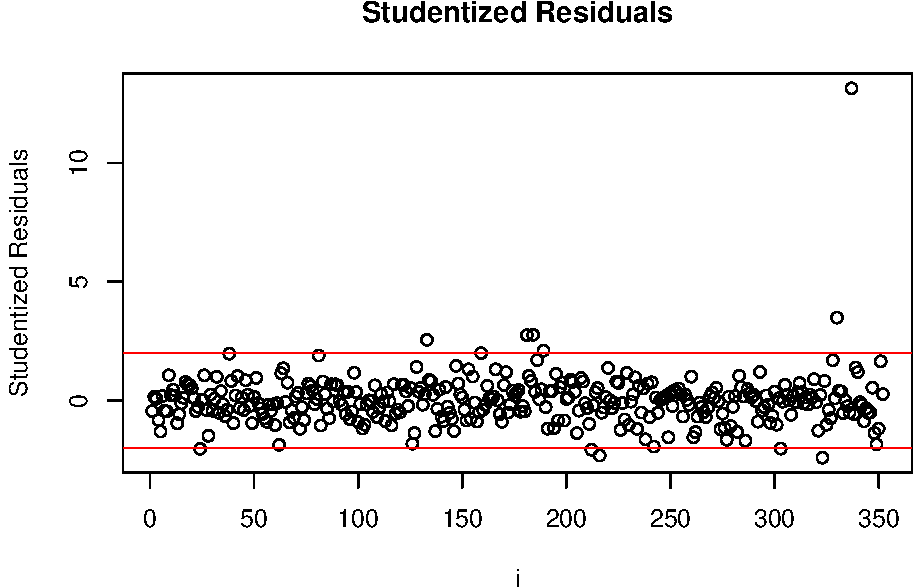
\includegraphics{project_files/figure-latex/unnamed-chunk-20-1.pdf}

\begin{longtable}[]{@{}llr@{}}
\toprule
county & state & Student Residuals\tabularnewline
\midrule
\endhead
Kings & NY & 13.144\tabularnewline
Atlantic & NJ & 3.490\tabularnewline
Wyandotte & KS & 2.763\tabularnewline
Ector & TX & 2.753\tabularnewline
Leon & FL & 2.553\tabularnewline
Delaware & IN & 2.406\tabularnewline
Jefferson & KY & 2.315\tabularnewline
Pulaski & AR & 2.097\tabularnewline
Worcester & MA & 2.069\tabularnewline
Monroe & IN & 2.033\tabularnewline
Columbiana & OH & 2.022\tabularnewline
Shawnee & KS & 1.995\tabularnewline
Clay & MO & 1.972\tabularnewline
\bottomrule
\end{longtable}

We can see from the Studentized residuals that there are a few notable
points. Kings county in NY is extremely far away from other points. We
compared models with and without Kings county but we found that keeping
Kings county in the data set had a better test mean squared error.

\subsubsection{DFBETA on continuous
coefficients}\label{dfbeta-on-continuous-coefficients}

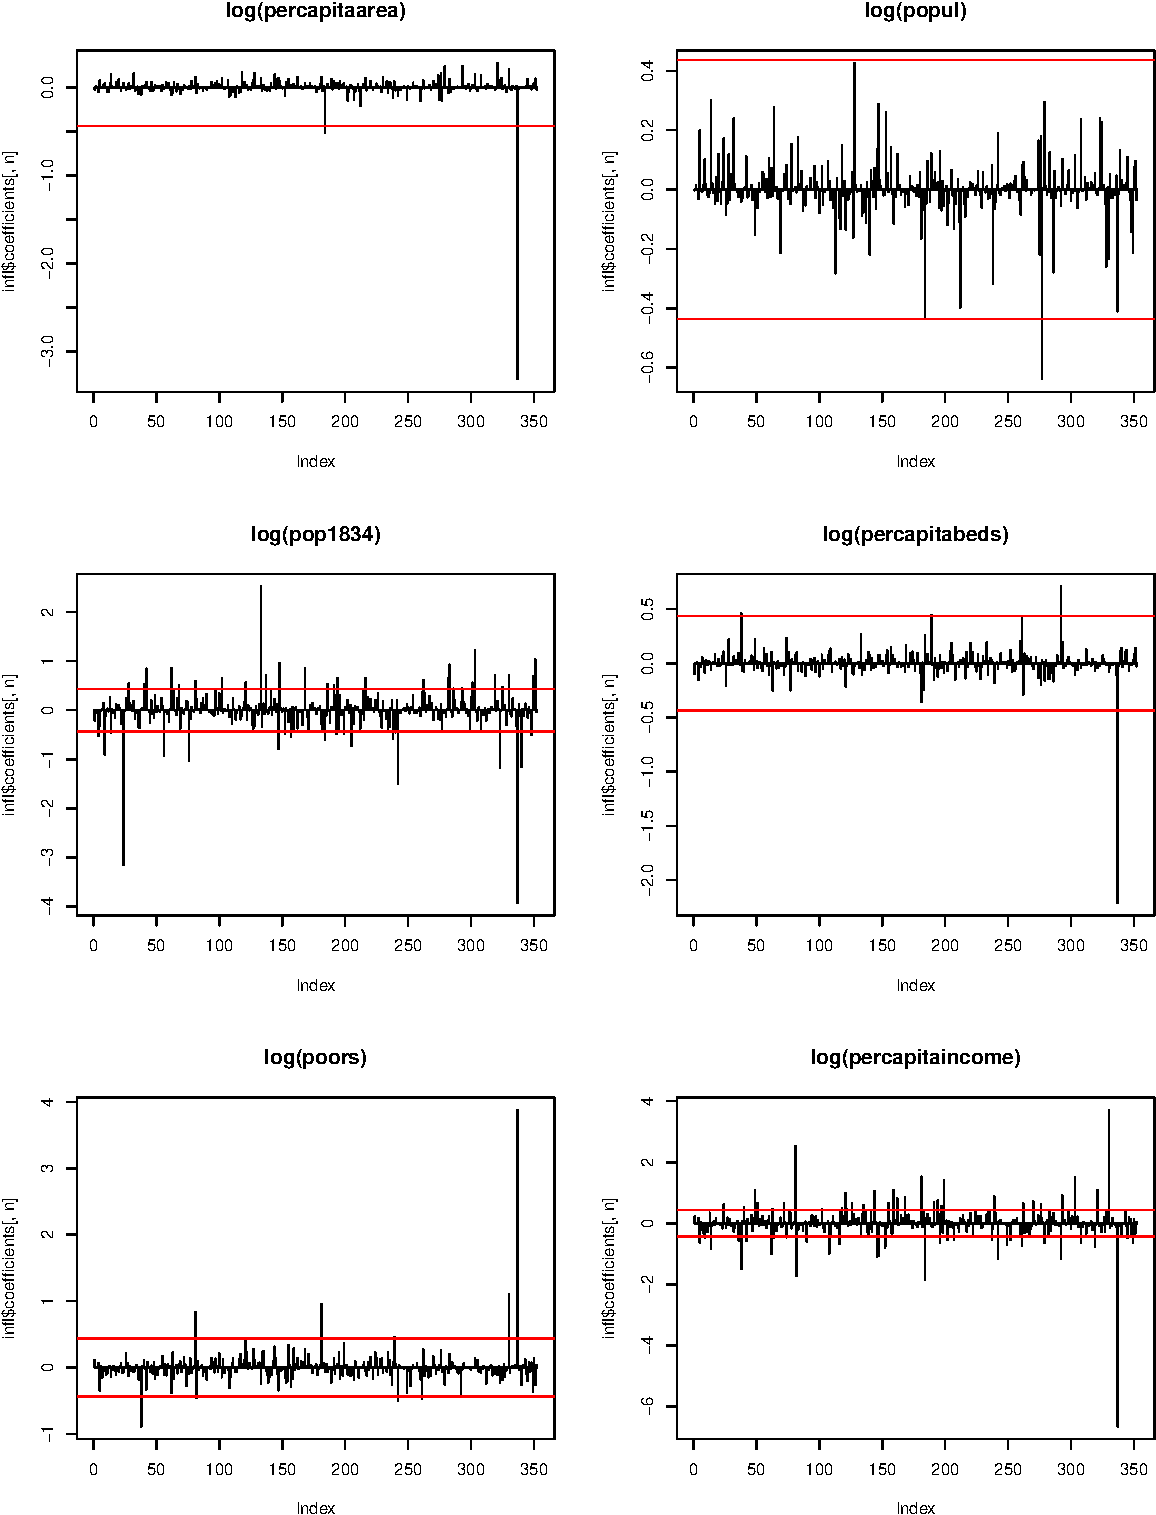
\includegraphics{project_files/figure-latex/unnamed-chunk-21-1.pdf}

\begin{longtable}[]{@{}llr@{}}
\toprule
county & coefficient & DFBETA\tabularnewline
\midrule
\endhead
Kings (NY) & log(percapitaincome) & -6.644\tabularnewline
Kings (NY) & log(pop1834) & -3.929\tabularnewline
Kings (NY) & log(poors) & 3.874\tabularnewline
Atlantic (NJ) & log(percapitaincome) & 3.704\tabularnewline
Kings (NY) & log(percapitaarea) & -3.317\tabularnewline
Monroe (IN) & log(pop1834) & -3.160\tabularnewline
Fulton (GA) & log(percapitaincome) & 2.537\tabularnewline
Leon (FL) & log(pop1834) & 2.521\tabularnewline
Kings (NY) & log(percapitabeds) & -2.209\tabularnewline
Wyandotte (KS) & log(percapitaincome) & -1.845\tabularnewline
Westchester (NY) & log(percapitaincome) & -1.723\tabularnewline
Ector (TX) & log(percapitaincome) & 1.527\tabularnewline
Pitt (NC) & log(pop1834) & -1.505\tabularnewline
Columbiana (OH) & log(percapitaincome) & 1.499\tabularnewline
Clay (MO) & log(percapitaincome) & -1.488\tabularnewline
Utah (UT) & log(percapitaincome) & 1.408\tabularnewline
Columbiana (OH) & log(pop1834) & 1.217\tabularnewline
Delaware (IN) & log(pop1834) & -1.171\tabularnewline
Fairfax\_County (VA) & log(percapitaincome) & -1.167\tabularnewline
Manatee (FL) & log(pop1834) & -1.148\tabularnewline
Pitt (NC) & log(percapitaincome) & -1.144\tabularnewline
Atlantic (NJ) & log(poors) & 1.102\tabularnewline
Shawnee (KS) & log(percapitaincome) & 1.098\tabularnewline
Philadelphia (PA) & log(percapitaincome) & 1.089\tabularnewline
San\_Mateo (CA) & log(percapitaincome) & -1.087\tabularnewline
\bottomrule
\end{longtable}

This table shows the sorted extreme \(DFBETA\) values for each of the
coefficients. Take for example Monroe (IN), which has a huge influence
on the \(pop1834\) parameter. If we look at the data, we see that Monroe
has 45.8\% of its population between 18 and 34. We see that Kings (NY),
influences many of the coefficients and has some of the most extreme
values. It is by far the most influential and extreme point in the data.

\paragraph{Model Diagnostic Plots}\label{model-diagnostic-plots}

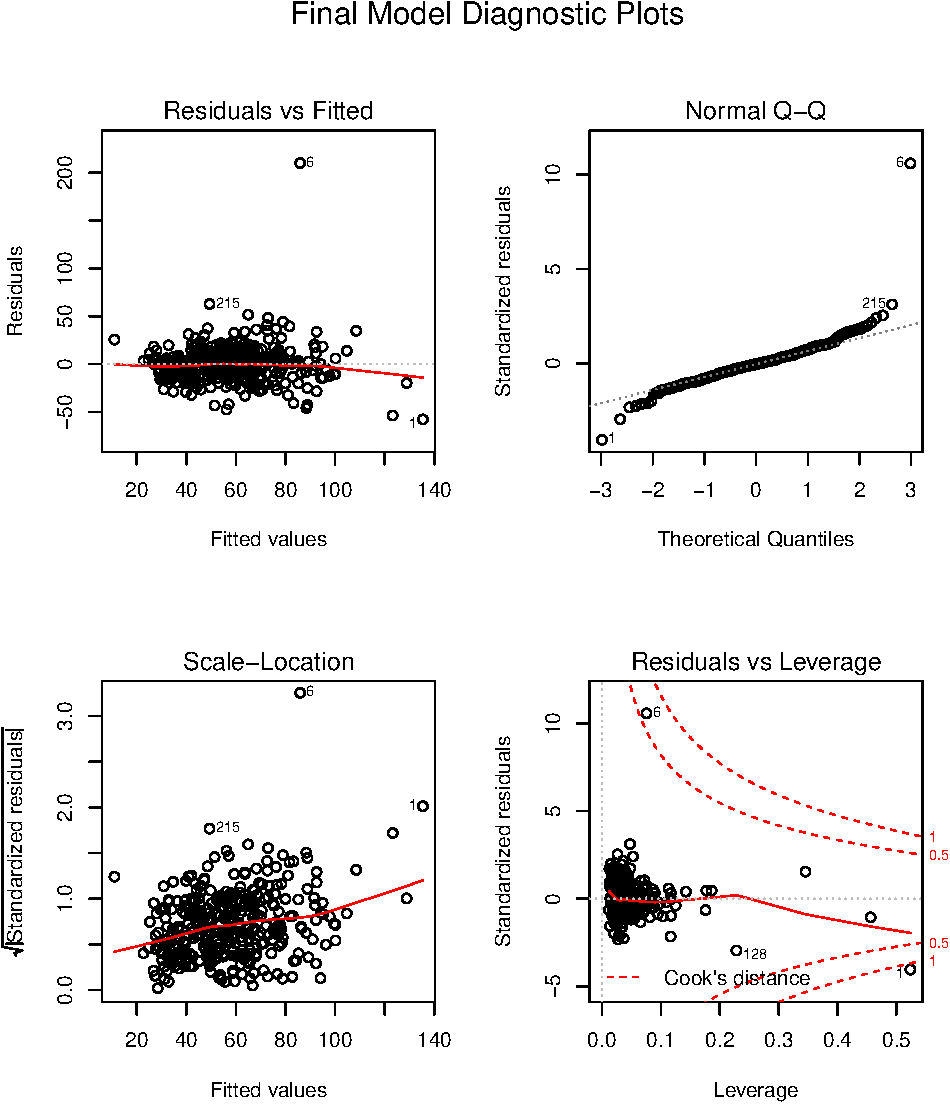
\includegraphics{project_files/figure-latex/unnamed-chunk-23-1.pdf}

We can see from the diagnostic plots that the residuals and fitted
values are approximately symmetric and the residuals don't appear to be
increasing or decreasing as the fitted values increases. The normal QQ
plot shows that we have larger tails than we would like. The estimates
for the parameters do not dependent on it following a normal
distribution but our p-values should be interpreted a little
pessimistically. The two points that are labeled, 6 (Kings) and 1 (Los
Angeles) are outliers. We can see that Los Angeles has a high leverage
and also an extreme standardized residual which makes it influential.
Kings county is closer to the mean for the dependent variables so it's
leverage is lower. It is still marked by the Residuals vs Leverage plot
as an issue as its residual is so high.

\subsubsection{Correlations}\label{correlations}

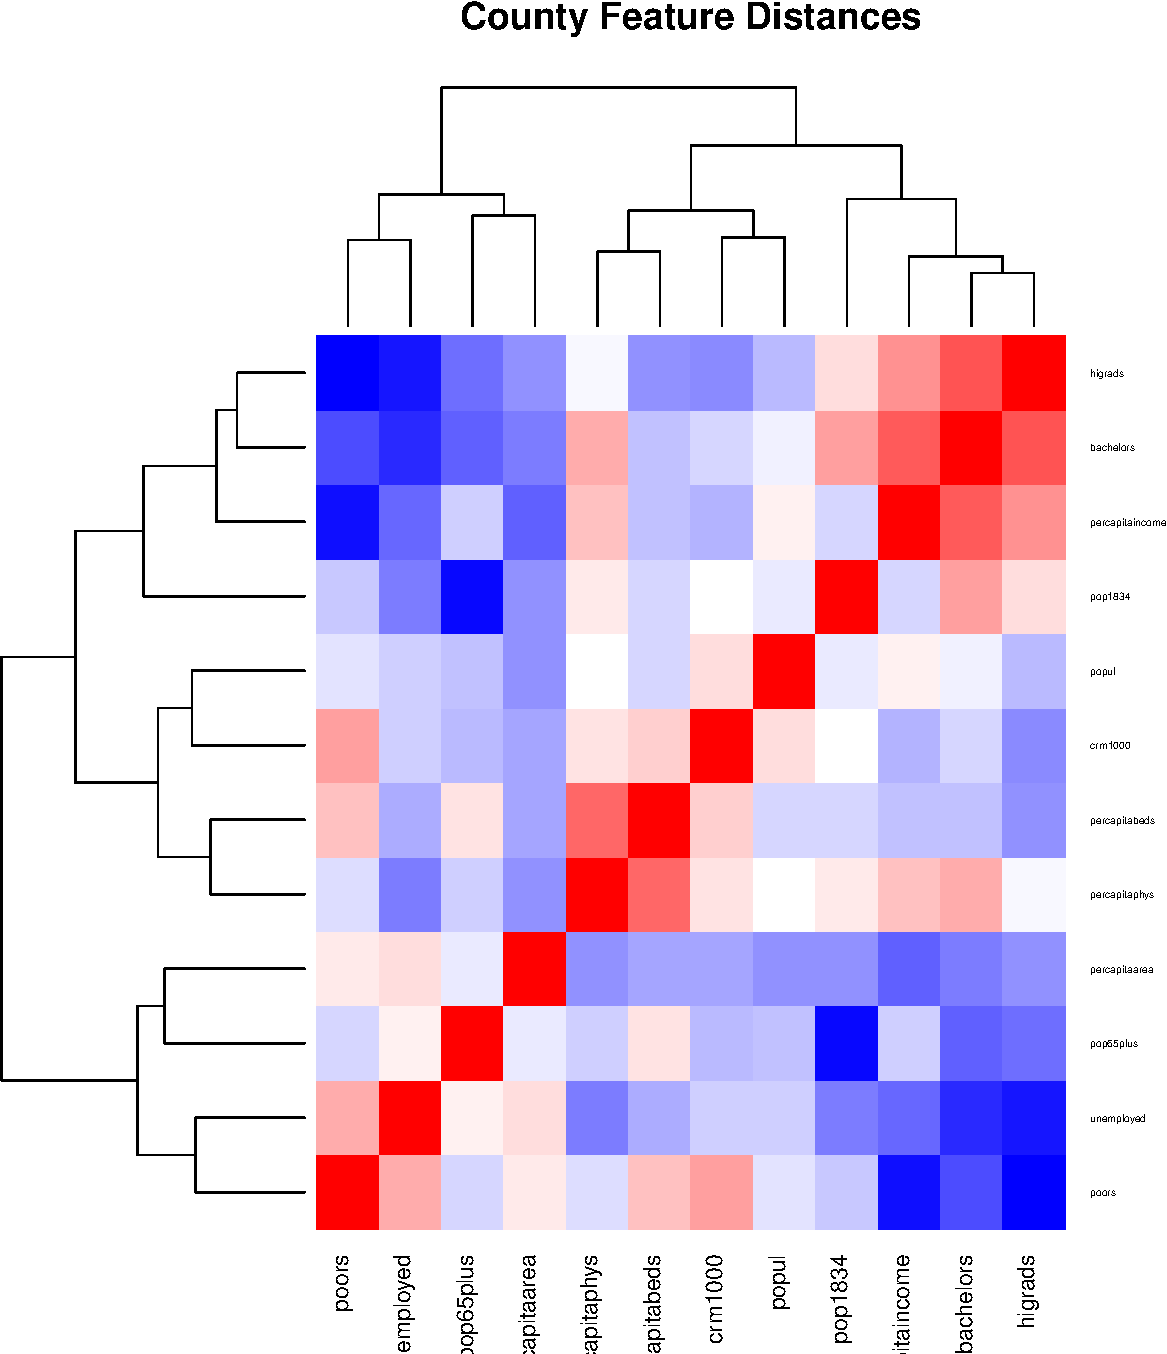
\includegraphics{project_files/figure-latex/unnamed-chunk-25-1.pdf} This
clustered distance matrix was how we selected which variables to remove
from the model. The blue variables are negatively correlated with each
other and the red variables are positively correlated.

\subsubsection{Outliers}\label{outliers-1}

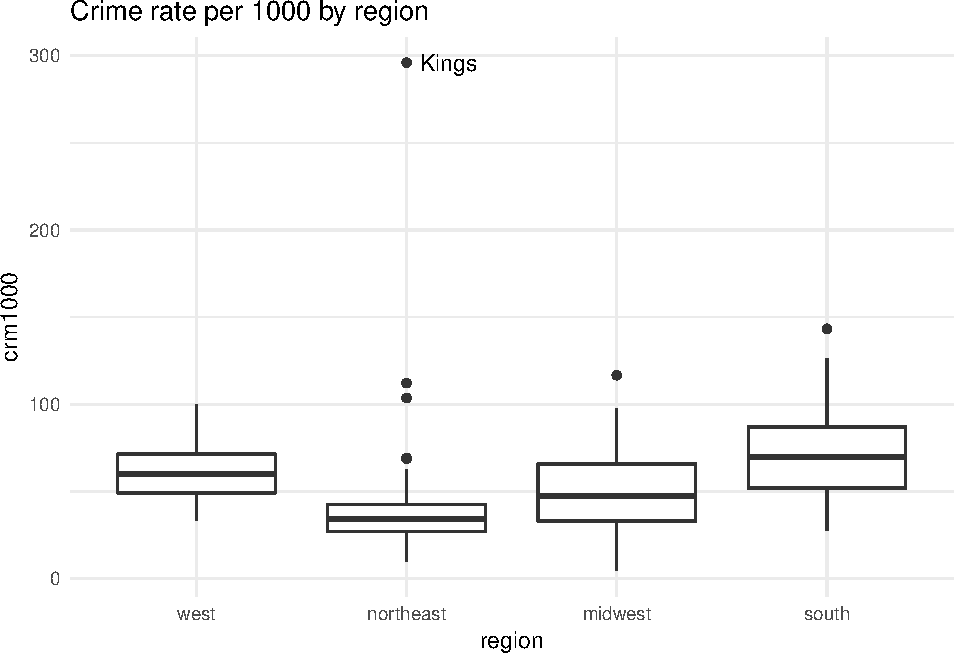
\includegraphics{project_files/figure-latex/unnamed-chunk-26-1.pdf} We
can see that Kings county is high for its region and overall.

\subsubsection{References}\label{references}

\begin{itemize}
\tightlist
\item
  \url{https://stats.idre.ucla.edu/stata/dae/negative-binomial-regression/}
\item
  ISL
\item
  Wikipedia: VIF, \ldots{}
\end{itemize}


\end{document}
